\documentclass[tikz,convert={outext=.svg,command=\unexpanded{pdf2svg \infile\space\outfile}},multi=false]{standalone}
\usepackage[utf8]{inputenc}
\usepackage{amsmath}


\begin{document}


\newcommand\colorboxsanssep[2]{{\colorbox{#1}{\hspace{-1mm}\ensuremath{{#2}\hspace{-1mm}}}}}

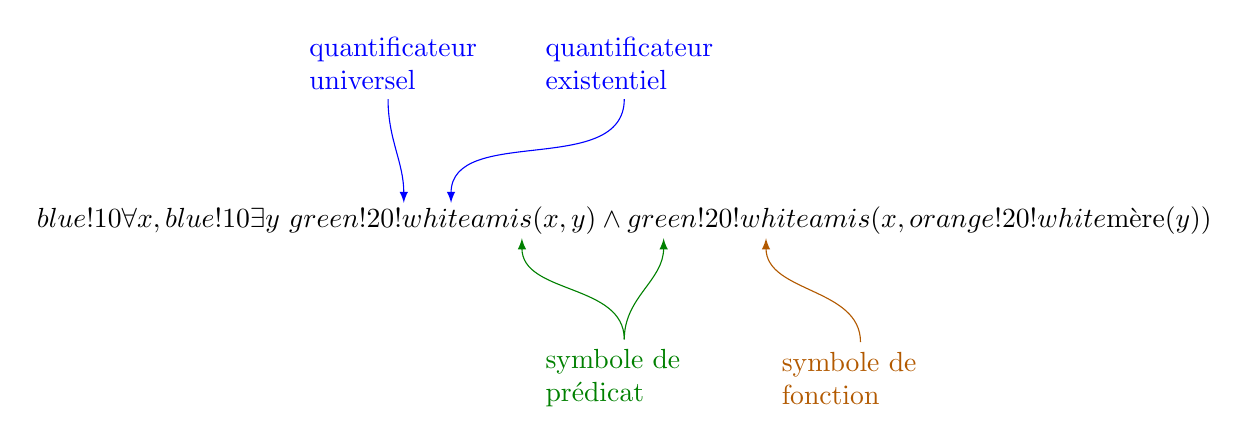
\begin{tikzpicture}
\tikzstyle{quanti}=[blue];
\tikzstyle{f}=[orange!70!black];
\tikzstyle{p}=[green!50!black];
\node[text width=2cm, quanti] at (-3,2) (forall) {quantificateur universel};
\node[text width=2cm, quanti] at (0,2) (exists) {quantificateur existentiel};

\node at (0,0) (formule) {$\colorboxsanssep{blue!10}{\forall}x, \colorboxsanssep{blue!10}{\exists}y ~ \colorboxsanssep{green!20!white}{amis}(x, y) \land  \colorboxsanssep{green!20!white}{amis}(x, \colorboxsanssep{orange!20!white}{\text{m\`ere}}(y))$};

\node[quanti] (formuleforall) at (-2.8, 0.1) {};
\node (formuleexists) at (-2.2, 0.1) {};
\node (formuleet) at (0, -0.1) {};
\node (formulef) at (1.8, -0.1) {};
\node (formulep1) at (-1.3, -0.1) {};
\node (formulep2) at (0.5, -0.1) {};
%\node at (0, 3) (variables) {variables};
%\node[text width=2cm] at (0, 2) (et) {connecteur booléen ``et''};
\node[text width=2cm, f] at (3, -2) (f) {symbole de fonction};
\node[text width=2cm, p] at (0, -2) (p) {symbole de prédicat};
\draw[-latex, quanti] (forall) edge [in=90, out=-90] (formuleforall);
\draw[-latex, quanti] (exists) edge[in=90, out=-90] (formuleexists);

\draw[-latex, p] (p) edge [in=-90, out=90] (formulep1);
\draw[-latex, p] (p) edge [in=-90, out=90] (formulep2);

\draw[-latex, f] (f) edge [in=-90, out=90] (formulef);


\end{tikzpicture}
\end{document}